\chapter{Software Methodology and Engineering Process}
\label{ch:methodology}

This chapter describes the software engineering process I followed
during my internship at FlowGenX AI: the development methodology, the
end-to-end development lifecycle of a feature, the version-control and
code-review workflow, the testing strategy, the metadata-generation
pipeline that takes a connector from source code to a live UI, and
the supporting toolchain.

The descriptions in this chapter are drawn from the project's
internal documentation and from my own day-to-day experience working
inside the process for five and a half months.

\section{Development Methodology}
FlowGenX AI follows a modern agile-inspired engineering process that
combines lightweight planning, asynchronous communication, and
continuous integration. Work is tracked on a \emph{ClickUp} board
where each connector or feature is represented as a card with status,
assignee, and links to the corresponding feature branch and pull
request. Tasks move through a typical kanban-style flow ---
\emph{To Do}, \emph{In Progress}, \emph{In Review},
\emph{Implemented}, \emph{API Tested}, \emph{MCP Playground Tested},
and \emph{Workflow Tested} --- giving the team end-to-end visibility
into where every feature is in its lifecycle.

In practice, the process I experienced has these defining
characteristics:

\begin{itemize}[leftmargin=*]
    \item \textbf{Incremental delivery.} Features are shipped as
    small, self-contained units (typically one connector at a time),
    each on its own branch and merged independently.

    \item \textbf{Asynchronous-first communication.} Most coordination
    happens through Google Chat threads and ClickUp comments. Live
    meetings are reserved for design discussions, code-walkthroughs,
    and blockers.

    \item \textbf{Reviewed everything.} No code reaches \texttt{dev}
    without a peer-reviewed pull request.

    \item \textbf{Automated enforcement of conventions.} Black,
    isort, Ruff, and pre-commit hooks reject style violations before
    code is even pushed.

    \item \textbf{Documentation as a deliverable.} A connector is
    not considered complete until it has both an integration test
    script and a UI Endpoint Test Reference document.
\end{itemize}

\section{End-to-End Development Lifecycle}
The lifecycle of a feature at FlowGenX AI --- specifically a new
connector, which was my primary unit of work --- moves through eight
distinct stages.

\subsection{Requirement Gathering}
A new connector is added to the platform either because a customer or
prospect needs it, or because the team is expanding the catalogue
strategically. Requirements are typically expressed as a ClickUp card
with the third-party platform name, its category (database, CRM,
finance, AI provider, and so on), the priority methods to expose, and
links to the third-party API documentation. The ClickUp board for the
connector backlog also tracks columns such as \emph{Available on UI?},
\emph{Auth Type}, \emph{Implementation Status}, \emph{API Tested},
\emph{MCP Playground Tested}, and \emph{Workflow Tested}.

\subsection{Design}
Before writing code, I would spend time reading the third-party API
documentation and identifying:

\begin{itemize}[leftmargin=*]
    \item The authentication pattern (API key, OAuth 2.0, basic auth,
    AWS IAM, and so on).
    \item The list of methods to expose (often dictated by what real
    workflows need).
    \item The pagination and rate-limiting model.
    \item The shape of request and response payloads.
    \item Any quirks (regional endpoints, multi-tenancy, async
    operations, file uploads).
\end{itemize}

This research output translates directly into the design of three
artefacts: the \texttt{ConnParams} Pydantic schema, the
\texttt{Manager} class, and the per-method modules.

\subsection{Implementation (the Development Cycle)}
A new connector lives under
\texttt{src/runtime\_connectivity/connectors/<name>/} and follows a
standardised three-tier architecture:

\begin{enumerate}[leftmargin=*]
    \item \textbf{Base managers (defined once in
    \texttt{connectors/base.py}):}
    \begin{itemize}
        \item \texttt{BaseManager} --- abstract foundation that
        defines \texttt{test\_connection}, \texttt{\_connect},
        \texttt{\_close}, and method introspection helpers used by
        the runtime to discover what a connector can do.
        \item \texttt{DBManager} --- adds standard database
        operations (\texttt{\_list\_tables},
        \texttt{\_read\_table\_as\_dataframe},
        \texttt{\_execute\_query\_to\_database},
        \texttt{\_write\_table\_to\_dataframe},
        \texttt{\_get\_table\_schema}).
        \item \texttt{FSManager} --- adds standard file-system
        operations (\texttt{\_list\_files}, \texttt{\_read\_file},
        \texttt{\_write\_file}, \texttt{\_delete\_file}).
        \item \texttt{ObjManager} --- the catch-all base class for
        object/API-based connectors (Salesforce, HubSpot, Stripe,
        and so on), where each connector defines its own custom
        methods.
    \end{itemize}

    \item \textbf{Connector implementation:}
    \begin{itemize}
        \item \texttt{\_\_init\_\_.py} exposes the connector's
        \texttt{ConnParams} Pydantic model, the \texttt{Manager}
        class, and the per-method imports.
        \item Individual method files (for example
        \texttt{create\_customer.py}) are decorated with
        \texttt{@openapi\_endpoint} and contain the business logic
        for that single endpoint.
        \item \texttt{test\_connection.py} validates that credentials
        actually work against the live API.
        \item \texttt{specs/} (for newer connectors) holds the
        auto-generated \texttt{connector\_metadata.json},
        \texttt{openapi\_spec.json}, and \texttt{auth\_config.json}.
    \end{itemize}

    \item \textbf{Connector registry:} every connector is registered
    in \texttt{connectors/\_\_init\_\_.py}, and the registry build
    is wrapped in a \texttt{try}/\texttt{except} so that a single
    broken connector cannot break the package import for everyone
    else.
\end{enumerate}

Every public method on a connector must be decorated with
\texttt{@openapi\_endpoint}. The decorator attaches OpenAPI metadata
(HTTP method, path, summary, parameters, request schema, response
schema, tags) that the platform later consumes to render the UI form
that end users see.

To support both synchronous and asynchronous callers, all connector
methods are wrapped using two utilities defined in
\texttt{runtime\_connectivity.utils}:

\begin{itemize}[leftmargin=*]
    \item \texttt{await dual\_method\_support\_from\_async(method, *args)}
    is used inside FastAPI handlers and other async contexts.
    \item \texttt{dual\_method\_support\_from\_sync(method, *args)} is
    used outside event loops and intentionally raises a
    \texttt{RuntimeError} if called from inside one.
\end{itemize}

\subsection{Code Review and Pull Requests}
Once a connector is implementation-complete, I would push the feature
branch and open a pull request against \texttt{dev}. Pull requests
follow a disciplined commit-message convention,
\texttt{feature/Rakib/(<connector>): <summary>}, so reviewers can
trace work per integration. Each PR is reviewed by at least one
senior engineer (typically my supervisor Abrar or the team lead
Sanjib). Reviewers comment line-by-line, request changes when the
\texttt{ConnParams} schema needs more validation, when an OpenAPI
example is missing, or when the test coverage is insufficient. A
typical PR goes through one or two rounds of review before being
merged.

When a teammate's changes had landed in \texttt{dev} between the time
I branched and the time I was ready to merge, I would rebase or
merge \texttt{origin/dev} into my branch and resolve conflicts
manually --- non-trivial conflict resolutions occurred on connectors
including AWS Textract, HelpScout, X (Twitter), Harness, Google Forms,
FreshBooks, Freshworks, and Zoho CRM.

\subsection{Testing Strategy}
Testing at FlowGenX AI happens at three layers.

\paragraph{Unit and contract tests.}
Each connector ships with \texttt{tests/connectors/test\_<name>.py}.
These tests use \texttt{pytest} fixtures and \texttt{unittest.mock}
to validate parameter validation, connection establishment,
DataFrame read/write operations, and error paths --- without making
real network calls.

\paragraph{Integration tests against the live API.}
For every connector I delivered, I additionally wrote a dedicated
integration test script under \texttt{scripts/} named
\texttt{test\_<connector>\_connector.py}. These scripts hit the
real third-party API with real credentials and produce a
\textsc{PASS} / \textsc{FAIL} / \textsc{SKIP} report per endpoint.
This is the single most important quality gate: it is what catches
authentication subtleties, pagination edge cases, schema drift in
the upstream API, and serialisation issues that mocked tests cannot
catch.

\paragraph{End-to-end UI and workflow validation.}
Once merged, every connector is validated through three additional
checks that are tracked on the ClickUp board: an
\emph{Implementation} review, an \emph{API Tested} pass, an
\emph{MCP Playground Tested} pass (Figure
\ref{fig:mcp-playground}), and a \emph{Workflow Tested} pass to
confirm it actually composes inside a real end-to-end workflow
(Figure \ref{fig:workflow-editor}).

\begin{figure}[H]
    \centering
    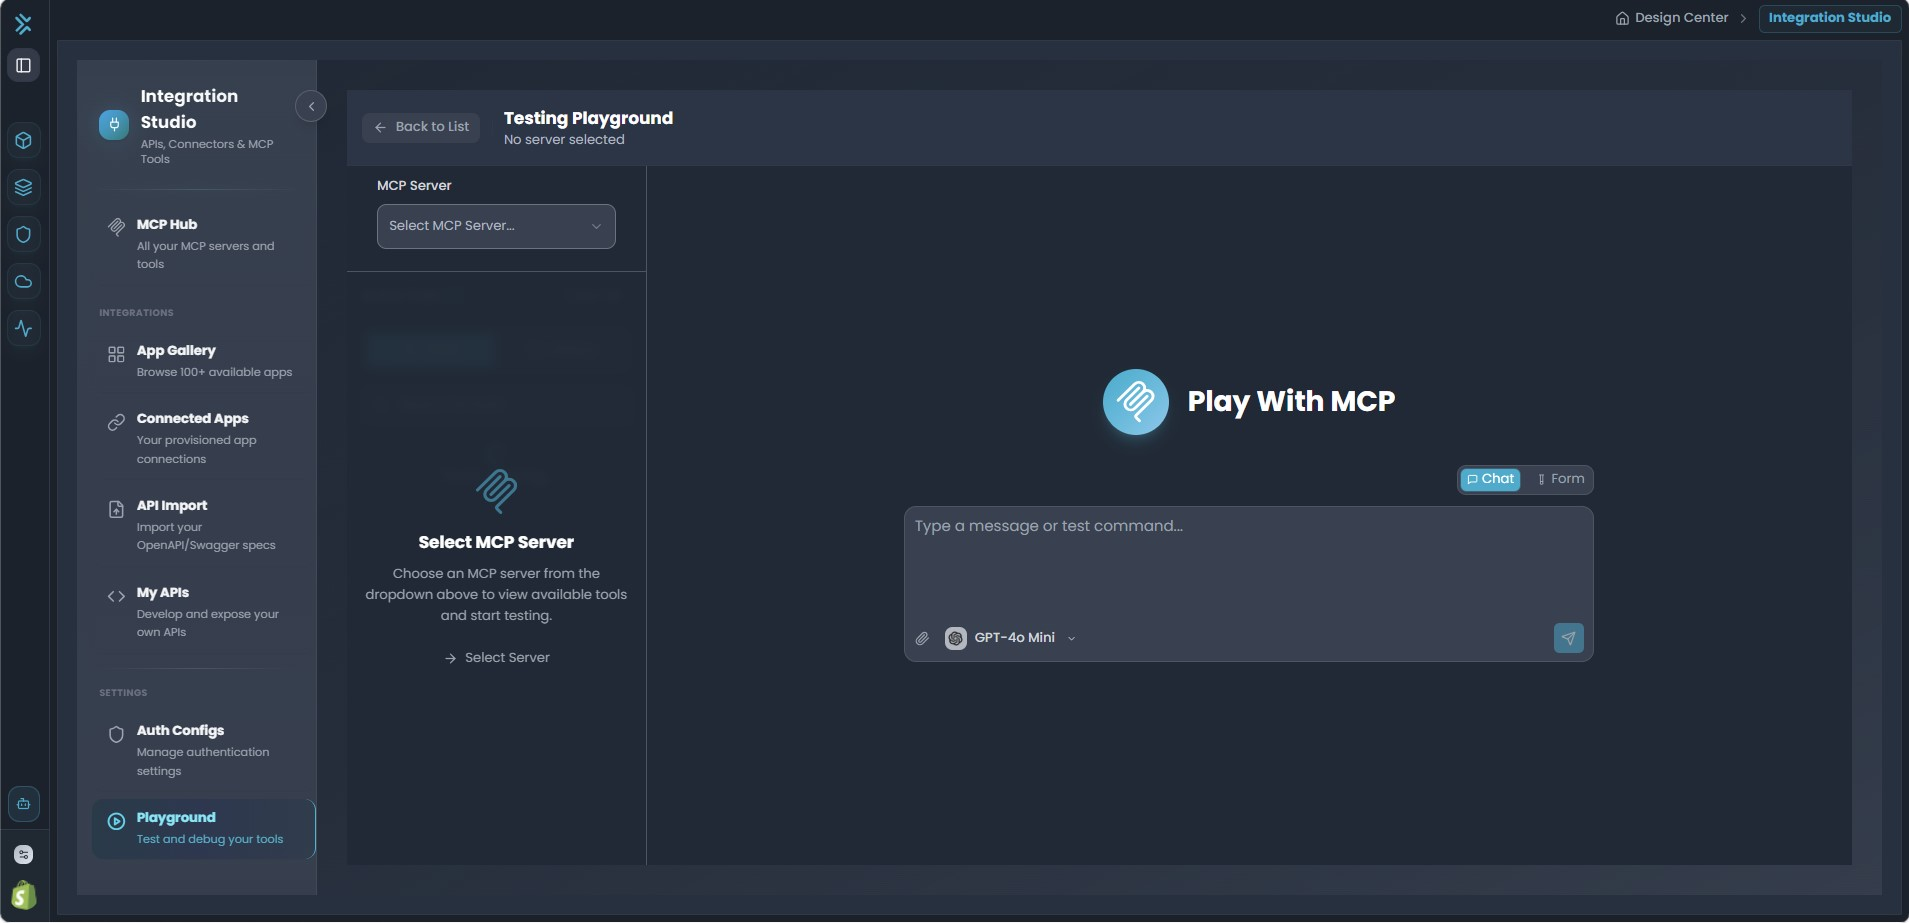
\includegraphics[width=0.95\textwidth]{figures/screenshots/MCP_playground.jpg}
    \caption{MCP Playground for end-to-end testing of connector tools.}
    \label{fig:mcp-playground}
\end{figure}

\subsection{Deployment to Development, Staging, and Production}
After a pull request is merged into \texttt{dev}, the change is
deployed to a development environment, where the team performs API
testing and end-to-end workflow validation. Once stable, the change
is promoted to a staging environment that mirrors production, and
finally to production. The platform itself is containerised with
Docker and orchestrated with Kubernetes, with infrastructure
provisioned through Helm charts and Terraform.

\subsection{Hotfixes}
Urgent production bugs are addressed outside the normal sprint
cadence through small, targeted patches that follow the same
review-and-test discipline as regular features but with a faster
turnaround. The specific hotfixes I contributed during the
internship are listed in Chapter~\ref{ch:activities}.

\section{Development Tools}
The lifecycle described above is supported by a small, consistent
toolchain. Source code lives in \textbf{Git} on \textbf{GitHub}, with
isolated feature branches scoped per connector and \texttt{dev} as the
integration branch from which environment promotions flow. Tasks are
tracked in \textbf{ClickUp}, where each connector card carries its
assignee, status, branch and pull-request links, and the four-stage
testing checklist (Implementation / API / MCP Playground / Workflow).
Code review happens inline on \textbf{GitHub Pull Requests}, where at
least one approval is required before merging. Python environments
are managed with \textbf{uv} (\texttt{uv pip install -e ".[dev]"});
runtime services are containerised with \textbf{Docker} and
orchestrated with \textbf{Kubernetes} (packaged via \textbf{Helm} and
provisioned via \textbf{Terraform}). API specifications are
\textbf{OpenAPI 3.0}, auto-generated from the
\texttt{@openapi\_endpoint}-decorated source code through
\texttt{generate\_openapi\_spec.py}. The team communicates through
\textbf{Google Chat} (asynchronous) and \textbf{Google Meet}
(synchronous); Microsoft Teams was used previously and was migrated
away from during my tenure.

\section{Error Handling and Logging Conventions}
The codebase imposes a small but strict convention for error handling
and logging:

\begin{itemize}[leftmargin=*]
    \item Errors raised inside a connector use
    \texttt{ConnectionExecutionError} (from
    \texttt{runtime\_connectivity.errors}) with a \texttt{message},
    \texttt{component} (set to \texttt{self.conn\_type}), and
    \texttt{method} parameter.
    \item Logging goes through the structured \texttt{app\_logger}
    from \texttt{runtime\_connectivity.logger}, with consistent
    \texttt{component} and \texttt{method} context, so log lines
    can be filtered cleanly per connector and per endpoint at runtime.
\end{itemize}